\documentclass{ttithesis}

\usepackage{amsmath}
\usepackage{graphicx}


\title{文間及びカテゴリ間の関係性を捉えた\\レーティング予測}
\author{12056\hspace{16ex}外山洋太}
\date{平成28年 2月}
\laboratory{知能数理研究室}



\begin{document}

\section{序論}

企業において商品の評判分析のためのレビューの評判分類は重要な問題である。
何万件という大量のレビューデータを人手で処理することは難しく、
計算機による自動化が望まれる。
その中で商品を複数のカテゴリにおいて分類をする問題がある。
カテゴリとは、宿泊施設のレビューを例にすると、サービス、立地、食事等の
レーティングが付けられる各項目のことである。
この問題に関する従来手法\cite{fujitani15}は、文間の関係性を考慮しておらず、
カテゴリ間については考慮しているものの深い関係性を捉えることができていない。

近年、その評判分類において、ニューラルネットワークを用いた手法が
提案されており、従来の手法を上回る分類精度を達成している。
ニューラルネットワークを分類問題に用いることの利点の一つは
層の数を増やすことによって
入力となる特徴量の深い意味を捉えることができることである。
多カテゴリの分類問題に適用すれば、
カテゴリ間の関係性を捉えた分類が実現できる。
さらに、文毎の特徴量を入力とすれば文間の関係性も捉えることができる。

文や文章の特徴量としては、パラグラフベクトル\cite{quoc14}が分類問題に対して
優れていることが示されている。

以上より、本研究では、複数カテゴリにおける評判分類について、
パラグラフベクトルとCNNを用いて文間及びカテゴリ間の関係性を捉えた分類を実現し、
従来手法から分類精度を向上させることを目的とする。



\section{関連研究}

\subsection{隠れ状態を用いたホテルレビューのレーティング予測}

藤谷ら\cite{fujitani15}は複数のカテゴリにおける評判分類問題に対して、
レビュー内の各文毎に予測した隠れレーティングから
レビュー全体のレーティングを予測する手法を提案している。
文毎のレーティングからレビュー全体のレーティングを予測する際の
カテゴリ間の繋がりを手動で変化させカテゴリ間の関係性を考慮している。

実験結果より、各文毎に隠れレーティングを予測することによって
分類精度が向上すること、
また、カテゴリ間の繋がりによって分類精度が変化することが示されている。


\subsection{パラグラフベクトル}

パラグラフベクトルは、文や文章といった大きな単位の言語表現の意味表現を
学習する手法である。これは、Continuous Bag Of Words
(CBOW)という単語の意味表現の 学習手法を応用した手法である。

以下に具体的なアルゴリズムを示す。
ここでは文章の意味表現を学習する場合について考える。
学習の概略を図\ref{fig:ParagraphVector}に示す。

まず、意味表現を学習する対象となる文に含まれる単語を
初めから一つずつ読んでいく。
その際、以下の式1に示す目的関数を最大化するように各パラメータの学習を行う。

\begin{gather}
  L = \frac{1}{T} \sum^{T - k}_{t = k} \log p(w_t | w_{t-k}, ..., w_{t+k}) \\
  p(w_t | w_{t-k}, ..., w_{t+k}) = \frac{e^{y_{w_t}}}{\sum_i e^{y_i}} \\
  y = b + Uh(w_{t-k}, ..., w_{t+k}, d; W, D)
\end{gather}

ここで、$d$は文、$w_i$は単語、$W$は全ての単語の分散表現を表す行列、
$D$は学習している全ての文章の分散表現を表す行列である。
$k$は片側のウィンドウサイズ、
$T$は現在の文章に含まれる単語数である。
$y$は現在の単語とウィンドウ内のその周りの単語及び現在の文章から導出される
対数確率である。 この値は、現在の単語とその文脈との類似度を表す。
$p$はsoftmax関数により正規化された、文脈から現在の単語が導かれることの
尤度である。

また、学習効率を高めるために、ネガティブサンプリングを行う場合がある、
ネガティブサンプリングとは、文脈外の単語をデータセットにおける出現確率で
サンプリングし、それらと文脈の意味が遠ざかるように$y$の式を決め
学習する手法である

これにより、Bag Of Words (BOW)と異なり、
単語の並び順を考慮した文や文章の分散表現を生成することができる。

\begin{figure}
  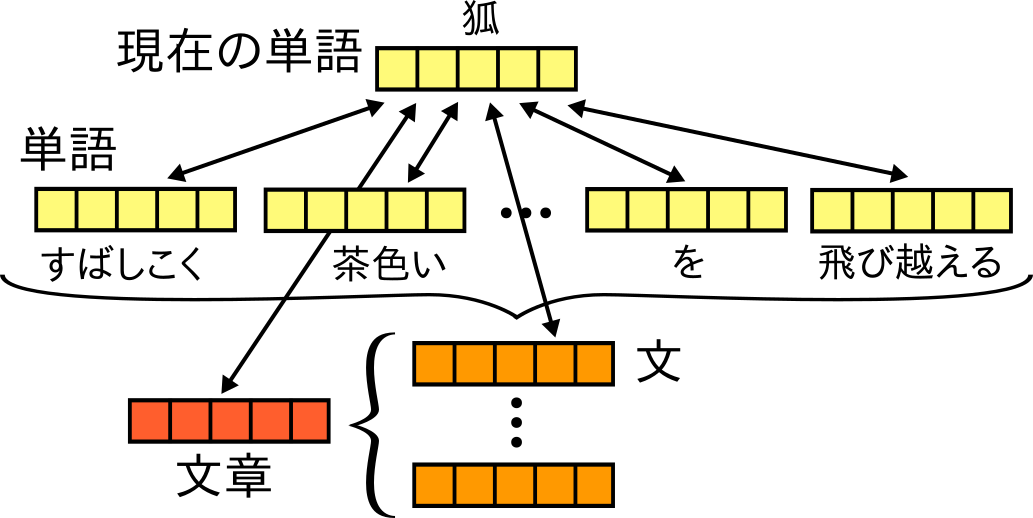
\includegraphics{fig/dvsvwv.png}
  \caption{文書及び文ベクトルの学習の概略}
  \label{fig:ParagraphVector}
\end{figure}

\section{提案手法}

提案手法では、パラグラフベクトルによってレビュー内の各文及び文章の分散表現を
生成し、それらをニューラルネットワークの入力として分類を行う。

\subsection{アイデア}

先行研究\cite{fujitani15}の実験結果から、
レビュー内の各文の特徴量を元にレビューの分類を行うことが
分類精度の向上に有効であると考えられる。
また、カテゴリ間の繋がりの変化が分類精度に影響していることから、
これをパラメータとして機械学習のモデルに組み込めば
分類精度を向上させることができると考えられる。

さらに、レビュー内の各文毎に分散表現を生成し分類器の入力とすることで、
その順序を考慮した学習を行う。
これにより、レビューの文章の大まかな文脈の流れが分類に利用できると考えられる。

\subsection{アルゴリズム}

初めに、パラグラフベクトルを用いて、
各レビューの文章とそれに含まれる各文のベクトルを生成する。
文章ベクトルと文ベクトルについては別々に生成する。

次に、各レビュー内の全ての文ベクトルに対して重み付け平均を行い、
圧縮された文ベクトルを生成する。
この過程により、各レビューで疎らだった文の数が統一される。
以下に重み付け平均を行う関数を示す。

\begin{gather}
w(x; w) = \frac{1}{2} (\cos(\frac{\pi |x|}{w}) + 1) \text{if $x$}
\end{gather}


提案手法に加え、基準手法としてNNへの入力となる特徴量が異なる4つの手法を用いた。
各手法に用いた特徴量を表\ref{tab:MethodFeatures}に列挙する。

\begin{table}
  \caption{各基準手法に用いた特徴量}
  \begin{tabular}{l | l}\label{tab:MethodFeatures}
    手法 & 特徴量 \\
    \hline
    基準手法  & レビュー全体の文書ベクトル \\
    提案手法1 & レビュー内で平均した文ベクトル \\
    提案手法2 & レビュー内で重み付け平均によって圧縮された文ベクトル \\
    提案手法3 & レビュー全体の文書ベクトル、レビュー内で平均した文ベクトル \\
    提案手法4 & レビュー全体の文書ベクトル、レビュー内で平均した文ベクトル \\
  \end{tabular}
\end{table}


\section{実験}

基準手法及び提案手法について分類精度を測定するために実験を行った。
全ての実験には、先行研究\cite{fujitani15}と同様に、
ホテル予約サイト楽天トラベルにおけるレビュー337,266件から
訓練データ300,000件、開発データ10,000件、評価データ10,000件を用いた。


\subsection{実験設定}

1つ目は各レビューに対する文書ベクトルのみを特徴量として用いたものである。
2つ目ははコメントの文書ベクトルに加え
コメント内の各文に対する文ベクトルの平均ベクトルを用いたものである。
一つ目と2つ目の基準手法の比較によって、
文書ベクトルに加え文ベクトルを用いることが有効であるかが示される。
2つ目の基準手法と提案手法の比較によって、
文の並び及びコメントの全体的なストーリーが分類に対して重要であるかが示される。

表XXXと表XXXに各手法でのパラメータ設定を示す。

\begin{table}
  \caption{文書ベクトルのみを用いた手法のパラメータ設定}
  \begin{tabular}{l | r}
    項目 & 値 \\
    \hline
    学習する単語の範囲 & 前後3単語 \\
    単語の最少出現回数 & 5 \\
    ベクトルの次元数 & 600 \\
    中間層の数 & 1 \\
    中間層でのニューロン数 & 512 \\
    入力層及び中間層でのドロップアウト率 & 0.2, 0.5 \\
  \end{tabular}
\end{table}


\subsection{結果}

表XXXに実験結果を示す。

\begin{table}
  \caption{実験結果}
  \begin{tabular}{l | r}
    手法 & 精度 \\
    \hline
    文書ベクトルのみを用いた手法 & 0 \\
    文書ベクトル及び平均した文ベクトルを用いた手法 & 0 \\
  \end{tabular}
\end{table}

\subsection{考察}

表XXXより、



\section{結論}

本研究では、レビュー全体の文書の分散表現に加え、
レビュー内の各文に対する分散表現の重み付き平均を用いた
評判分類の手法を提案した。

実験により、従来手法\cite{fujitani15}及びレビュー全体の文書ベクトルのみを用いた手法に比べ、
提案手法が高い分類精度を示すことが分かった。
同時に、これはレビュー内の文の並びが評判分類に重要であることを示す。



\subsection{今後の課題}

今後の課題は、2つに分かれている学習モデルの統一である。

提案手法は、分類すべき文書とそれが含む文の分散表現を生成する段階、及び、
それらを用いて分類を行う段階の2つの段階に分かれている。
このことは、問題を2つに分けることで個々の問題を単純にしているが、
同時に一つずつ文書の分類を行うことを難しくしている。
また、提案手法において、文書や文の分散表現を事前に生成するための
パラグラフベクトルの手法におけるパラメータは、
実際には最大の分類精度を達成するため分類器のパラメータとして最適化されることが
望ましい。

今後は、これらの問題を解決するために、文書や文の分散表現を生成する過程を
ニューラルネットワークによる分類器に取り込む。
これによって、学習方法の柔軟性を高めると共にさらなる分類精度の向上を目指す。




\begin{thebibliography}{9}
\bibitem{fujitani15}
  藤谷宣典ら,
  隠れ状態を用いたホテルレビューのレーティング予測.
  言語処理学会第21回年次大会, 2015.
\bibitem{quoc14}
  Quoc Le, and Tomas Mikolov,
  Distributed Representations of Sentences and Documents.
  ICML 2014, 2014.
\bibitem{nal14}
  Nal Kalchbrenner, Edward Grefenstette, and Phil Blunsom,
  A Convolutional Neural Network for Modelling Sentences.
  ACL 2014, 2014.
\bibitem{rie14}
  Rie Johnson, and Tong Zhang,
  Effective Use of Word Order for Text Categorization
  with Convolutional Neural Networks.
  NAACL 2015, 2015.
\bibitem{duyu15}
  Duyu Tang, Bing Qin, and Ting Liu,
  Learning Semantic Representation of Users and Products
  for Document Level Sentiment Classification.
  ACL 2015, 2015.
\end{thebibliography}

\end{document}
